\documentclass[sigconf,anonymous,review]{acmart}
% For citations
%\usepackage[sort,numbers]{StyFiles/natbib}
% \setcopyright{rightsretained}
% \settopmatter{printacmref=false}
\acmSubmissionID{1486}

%%
\usepackage{graphicx}
% \usepackage{url}

% \usepackage{pifont}
% \newcommand{\cmark}{\text{\ding{51}}}
% \newcommand{\xmark}{\text{\ding{55}}}
% \usepackage{amssymb}
% \newcommand{\RN}[1]{%
%   \textup{\uppercase\expandafter{\romannumeral#1}}%
% }
% DOI
%\acmDOI{10.475/123_4}
% ISBN
%\acmISBN{123-4567-24-567/08/06}

%%

\renewcommand{\citename}{\citet}
\renewcommand{\cite}{\citep}

% For maths
\usepackage{amssymb}

% For algorithms
\usepackage{StyFiles/algorithm}
\usepackage{StyFiles/algorithmic}

% My macros
\usepackage{StyFiles/sg-macros}

\newtheorem{thm}{Theorem}[section]
\newtheorem{cor}[thm]{Corollary}
\newtheorem{lem}[thm]{Lemma}
\newtheorem{prop}[thm]{Proposition}
\newtheorem{obs}[thm]{Observation}
\newtheorem{defn}[thm]{Definition}

\newcommand{\mmqp}[3]{\textrm{\sc MaxMarginQP}\!\left(\{\by_t, #1\}_{t=1}^{T}, #2, #3\right)}

% MISC
\usepackage{textcomp}
\usepackage{makecell}
\usepackage{booktabs}
\usepackage{multirow}

%Conference
 \acmConference[KDD 2019]{}{August 3-7 2019}{Anchorage, Alaska USA}
 \acmYear{2019}
 \copyrightyear{2018}

\begin{document}

\title[Multi-task RNN and Higer-order MRFs for Stock Price Prediction]{Multi-task Recurrent Neural Network and
  Higher-order Markov Random Fields for Stock Price
  Prediction}

% \numberofauthors{3}

% \author{
% \alignauthor Chang Li \\
%       \affaddr{UBTECH Sydney AI Centre, SCS, University of Sydney}\\
%       \email{chli4934@uni.sydney.edu.au}
% \alignauthor Dongjin Song \\
%       \affaddr{NEC Laboratories America, Inc.}\\
%       \email{dsong@nec-labs.com}
% \alignauthor Dacheng Tao\\
%       \affaddr{UBTECH Sydney AI Centre, SCS, University of Sydney}\\
%       \email{dacheng.tao@sydney.edu.au}
% }
% \date{15 Jan 2019}


\begin{abstract}
  Stock price movement not only depends on individual stocks'
  historical records, but also has complex hidden dynamics associated with other correlated stocks. Despite a substantial amount of effort has been made to understand the principles of stock price movement, few has attempted to perform stock price prediction based upon
  single stock's historical records as well as its correlated stocks. To this end, we present a multi-task recurrent neural network (RNN) and high-order Markov random fields (MRFs) to perform stock price prediction. Specifically, we first design a multi-task RNN framework to extract informative features from the raw market data of individual stock without considering any domain knowledge. Next, we employ binary MRFs with
  unary as well as weighted lower linear envelope as the higher-order energy
  function to capture the higher-order consistency within the same clique (group) of stocks. We also derived a latent structural SVM algorithm to learn high-order MRFs in a
  polynomial number of iterations. Finally, a sub-gradient
  algorithm is employed to perform end-to-end training of RNN and
  high-order MRFs. We conduct thoroughly empirical studies based on three popular Chinese
  stock market indexes and the proposed method outperforms baseline approaches. To the best of our knowledge, the proposed technique is the first one to
  investigate intra-clique relationships with higher-order MRFs on stock price prediction.
\end{abstract}

\keywords{Deep learning, Multivariate time series prediction, High-order Markov random fields}

\maketitle

\section{Introduction}
\label{sec:intro}
% lead lag 现象不是一直存在,个股趋势也非常重要

It has been well-known that single stock's price movement not only depends on its historical records, but also is highly correlated to other stocks~\cite{lo1990contrarian,mech1993portfolio} and may change in a non-synchronous
manner~\cite{lo1990contrarian,brennan1993investment}. This correlated yet asynchronous price movement phenomenon is sometimes defined as lead-lag relationship~\cite{hou2007industry} within a group of stocks.
Different speed of information diffusion has been believed to be
the main reason of lead-lag relationship
\cite{lo1990contrarian,badrinath1995shepherds,mcqueen1996delayed}.
When an information hits the market, some stocks\textquotesingle price tend to
react faster than others. Therefore, identification of those
leading stocks and their lead-lag relationships to other lagging
stocks will provide strong evidence in predicting the latter\textquotesingle s
price movement direction.

There are three key challenges in utilizing the lead-lag relationship: (1) Analyzing which group of stocks ($e.g.$, industry,
supply chain, $etc.$) will be affected by newly arrived information
and the corresponding leading stocks; (2) Identifying lagging stocks in this group and modeling their relationships; (3) Predicting
price movement of each stock by jointly considering the knowledge in its correlated group and individual stock\textquotesingle s price movement at current stage.

The first challenge is extremely difficult to resolve with an automatic algorithm. This is not only because it requires an expert level understanding of the finance system and the dynamics behind market news as well as stock price, but also due to lacking of training data. However, according to the well-known efficient market hypothesis~\cite{malkiel1970efficient}, stock price reflects all
available market information. Therefore, informative stock price changes can be employed as an proximity to market news arrival. In this way, the complexity of the first challenge is transformed to the detection of informative price changes in individual stock.

Economists have spent decades trying to use patterns hidden
inside historical trading price and volume to predict future
price movement~\cite{fama1966filter,jensen1967random}. Those
models are called technical
analysis~\cite{kirkpatrick2010technical}. However, most of those
models have been proven stopped generating profitable signals
since the early 1990s~\cite{park2007we}. On the other hand, since
trading strategies based on technical analysis rules are public
available and easy to replicate, informed institutional traders
are motivated to manipulate market price and trap retail
(individual) traders following their manipulated price to gain
excess profit~\cite{sun2016decision}.

To overcome those problems and address the first challenge, we employ an end-to-end
hierarchical multi-task~\cite{caruana1993multitask} RNN to
extract informative changes from raw market price without using
any of hand-crafted features such as technical analysis
indicators. Good performance on price prediction relies on rich
representations as well as the multi-task framework which can leverage
complementary aspects from diverse tasks~\cite{sogaard2016deep}. Specifically, given the raw market price data which only contains six features ($i.e.$, opening
price, low price, high price, closing price, volume, and amount) at each time interval, we leverage a hierarchical multi-task
network to extract features on different tasks first and then concatenate those complementary feature vectors to make final prediction.

To model lead-lag relationships and address the other two challenges, we present a
binary Markov Random Fields (MRFs) with weighted lower linear envelope as higher order (when the clique contains more than two
nodes) energy function~\cite{Kohli:CVPR07,Nowozin:2011,Gould:ICML2011,gouldlearning}.
In our implementation, we treat each stock as a node in MRFs and each stocks group which has lead-lag relationships as a maximum clique in MRFs. We use pre-defined industry classification
list~\cite{ths} as the prior domain knowledge of each stock\textquotesingle s belonging maximum clique. Finally, the
complexity of modeling dynamics between leading and lagging stocks becomes encouraging consistent over large cliques under
weighted lower linear envelope potentials. Logits from hierarchical RNN networks are used as unary features in MRFs. By minimizing the energy function which contains both unary and higher order
features, we are able to predict each stock\textquotesingle s future price movement by jointly considering individual market
price trending together with lead-lag relationships.

We justify the effectiveness of the proposed technique based on three popular Chinese stock market indexes and the proposed method outperforms baseline approaches. To the best of our knowledge, the proposed technique is the first one to investigate intra-clique relationships with higher-order MRFs on stock price prediction.
  
%We verify our methodology on Chinese stock market because
%it is generally considered less mature than other developed
%countries\textquotesingle thus potentially to be more
%profitable~\cite{bessembinder1995profitability}. Even though immature, \citename{fangyan2012} found that the average duration of information arrival-conduction-integration-release process is $4.04$ minutes. Therefore, a minute-level frequency model ismandatory to leverage from lead-lag relationship. To our best knowledge, our model is the first one demonstrating lead-lag relationship at minute-level frequency on Chinese stock market.

To summarize, the main contributions of this paper include: 
\begin{itemize}
\item  We propose a hierarchical multi-task RNN architecture to learn stock price
patterns without any hand-crafted feature.
\item We propose the first model that encode lead-lag relationship among stocks using
higher-order MRFs. 
\item We develop an algorithm to learn weighted lower linear envelope with latent variables as higher order energy function under latent structural SVMs framework. Adding latent variable into higher order function
enables our model to learn much richer representation than
previous study~\cite{gouldlearning}.
\end{itemize}

\section{Related Works}
\label{sec:background}
This work is closely related to lead-lag relationship, multi-task learning, high-order MRFs, as well as latent structural SVMs.

\textbf{Lead-lag relationship} Lead-lag relationship has been found to be a long existence phenomenon in stock market. Many reasons can lead to it such as diffusion of information, sector (industry) rotation, investment style rotation, event driven trading and asynchronous trading
\cite{lo1990contrarian,chordia2000trading,conrad1988time,hameed1997time}. Generally it is believed that lead-lag relationship is more prevalent for firms in the same industry \cite{hou2007industry}. This assumption gives rise to our setting that we use pre-defined industry classification list \cite{ths} as prior domain knowledge of each stock\textquotesingle s belonging maximum
clique. A lot of research \cite{brennan1993investment,hou2007industry,badrinath1995shepherds,mcqueen1996delayed}
indicates that stocks with larger capital size and higher liquidity tend to be leading stocks and vice versa.
To replicate potential lead-lag relationship, we assign each stock a different weight from its corresponding indexes created by the China Securities Index Company, Ltd. More complicated dynamics hidden behind clique
of stocks are learned by higher-order MRFs.

\textbf{Multi-task learning} \citename{caruana1993multitask}
showed that inductive knowledge learned from multiple tasks can
transfer between tasks and help improving generalization on all
tasks. Many works in Natural Language Processing (NLP) area take
advantage of multi-task framework and achieves state-of-the-art
performance while using simple models for each of these tasks
\cite{sogaard2016deep,hashimoto2016joint}. However, as pointed
out by many researchers
\cite{caruana1993multitask,ruder2017overview}, there are lacking
of theories on choosing a diverse set of tasks and hierarchical
architecture of chosen tasks. Recent works
\cite{sogaard2016deep,hashimoto2016joint} apply the intuition
that the complexity of task should be increasing along with
hierarchical level. We follow this intuition in our
implementation. Because technical analysis indicators can be
categorized into four categories (trend, momentum, volatility and
volume)~\cite{kirkpatrick2010technical} and volume is included in
market price data, we propose an architecture that using trend
and volatility tasks as our lower level tasks and price movement
classification (upward or downward) as higher level task. Other
selection of tasks and hierarchical designations remain open for
further research.


%\textbf{Graphical model and neural networks} It has been known that neural networks are lacking of constraints enforcing label consistency. There are many efforts demonstrating this issue by combining CRFs and neural networks. From natural language processing community, \citename{collobert2011natural} proposed a CRF on top of feed-forward neural networks for constituency parsing task (Part-Of-Speech tagging e.g.). Due to the fixed sized window, their method only provides local information to CRF without long-term memory. For the same task, \citename{huang2015bidirectional} proposed a Bi-LSTM-CRF framework which utilizes both forward and backward information by using LSTM to extract features from raw text and make inference at a sentence level by using CRF. They achieved a more robust model and outperformed previous study. Later works~\cite{ma2016end,lample2016neural} follow their routine and improved bottom neural networks to encode both character-level and word-level features without using hand-crafted features. However, CRF they use still remains sequential. Computer vision community also put many efforts in combining benefits of Neural Networks and CRF \cite{chen2018deeplab,zheng2015conditional}. \citename{zheng2015conditional} formulated fully connected CRF with Gaussian edge potentials and mean-field inference as RNNs and integrated it into CNNs. The CRF-RNNs network can be optimized using standard back-propagation method.

%One main drawback of all above frameworks is that they only use unary and pairwise potentials. To include higher-order potentials, \citename{arnab2016higher} extends previous work by designing two types of potentials which can be formulated into CNNs when using mean-field inference. However, mean-field inference is an approximation inference method and choices of potentials are very limited under this kind of formulation. \citename{witoonchart2017application} proposed a variety of construction of graphical model and neural networks. They use graph-cut like algorithm to calculate loss-augmented inference during forward propagation of graphical models and back-propagate the error learned with Structured SVMs \cite{Joachims:ML09} to CNNs. In this paper, we follow their back-propagation method and implement an end-to-end training framework for learning higher order MRFs and neural networks using latent structural SVMs \cite{yu2009learning} algorithm.


\textbf{Higher-order Markov random fields} Markov random
  fields are also known as undirected graphical model
that can be seen as a regularized joint log-probability
distribution of arbitrary non-negative functions over a set of
maximal cliques of the graph~\cite{bishop:2006:PRML}. Utilizing
MRFs mainly involves three steps: defining energy
  functions, solving inference problem (MAP or energy
minimization) and learning parameters. As for energy
  functions, our work focus on a class of higher-order
potentials defined as a concave piecewise linear function which
is known as lower linear envelope potentials over a clique
of binary variables. It has been raising much interest due to its
capability of encoding consistent constraints over large subsets
of pixels in an image~\cite{Kohli:CVPR07,Nowozin:2011}. We follow
\citename{gouldlearning} to construct a graph-cut algorithm to
solve exact inference problem and propose our novel learning
algorithms under latent structural SVM in
section~\ref{sec:learning}.

As the second step, in order to solve inference problem,
\citename{kohli2009robust} proposed a method to represent a class
of higher order potentials with lower (upper) linear envelope
potentials. By introducing auxiliary
variables~\cite{Kohli:CVPR10}, they reduced the linear
representation to a pairwise form and proposed an approximate
algorithm with standard linear programming methods. However, they
only show an exact inference algorithm on at most three terms.
Following their routine, \citename{gouldlearning} extended their
method to a weighted lower linear envelope with arbitrary many
terms which can be solved with an efficient algorithm. They
showed the energy function with auxiliary variables is submodular
by transforming it into a quadratic pseudo-Boolean
form~\cite{Boros:MATH02} and how
graph-cuts~\cite{Hammer:1965, Boykov:ICCV01,
  Freedman:CVPR05} like algorithm can be applied to do exact
inference.

As the third step, \citename{gouldlearning} solved
learning problem of lower linear envelope under the max
margin framework~\cite{tsochantaridis2005large}. In their work, 
they pointed out the potential relationship between their
auxiliary representation and latent SVM~\cite{yu2009learning}.
Our work is closely based on their research. We continue to use
the higher order energy function and inference algorithm
developed in their previous work~\cite{Gould:ICML2011} and extend
their max margin learning algorithm to include latent variables.
The learning algorithm we use is an extension of max margin
framework which is known as ``latent structural
SVM''~\cite{yu2009learning}.

\textbf{Latent structural SVMs} The max-margin
framework~\cite{Taskar:ICML05,tsochantaridis2005large} is a
principled approach to learn weights of pairwise MRFs.
\citename{Szummer:ECCV08} adapted this framework to optimize
parameters of pairwise MRFs inferred by graph-cuts method. In
order to adapt higher-order energy function to max margin
framework, \citename{Gould:ICML2011} approximated the energy
function using equally spaced break-points.
\citename{gouldlearning} extended this framework with additional
linear constraints which enforces concavity on weights thus can
be used for learning lower linear envelope potentials. However,
those methods can only learn higher-order functions
approximately. In this paper we propose an algorithm to optimize
the energy function exactly by introducing auxiliary variables
back into the feature vector and solving the learning problem
using the latent structural SVM framework
~\cite{yu2009learning}. To include unobserved information,
\citename{yu2009learning} extended the joint feature function in
structural SVM with latent variables and re-write the object
function of SSVM into a difference of two convex functions.
Problem of this formulation can be solved using the
Concave-Convex Procedure (CCCP)\cite{yuille2002concave} which is
a two stages algorithm and guaranteed to converge to a local
minimum.

% At the first step latent variables which best explains training
% pair is found by solving ``latent variable completion''
% problem. At the second step inferred latent variables are used
% as completely observed. Therefore, solving object function with
% latent variables reduces to solve the standard structural SVM
% problem.

The latent structural SVM cannot take input data directly such
as structural SVM. In order to use it, inference algorithm, as
well as the MRF feature function, loss function, and latent
variable completion problem\cite{yu2009learning} need to be
implemented first. Our implementation is described in
section~\ref{sec:opt}.

\section{Methods}
\label{sec:meth}

In this section, we introduce multi-task DNNs-MRFs architecture
from lower part to the top part. The whole model is constructed
with two parts. The first part is a ``Holistic Market Price
Learner'', which contains three DARNN modules. The goal of the
first part is to extract informational representations of raw
market price end-to-end without any input of hand-crafted
features and technical indicators from stock market. The second
part is called ``Section Rotation Predictor'' which is a binary
Markov Random Fields model contains higher order energy
functions. Those higher order functions are applied to financial
experts defined sector lists (used as maximum cliques). The goal
of this part is to utilizing unary features learned by DNNs
together with domain knowledge from financial experts by modeling
higher order consistency among stocks which belong to the same
sector. We summarized the whole architecture in
figure~\ref{fig:mrfrnn}.


\subsection{Holistic Market Price Learner}
\label{sec:hmpl}

The ``Holistic Market Price Learner(HMPL)'' contains two levels,
three modules of DARNNs\cite{qin2017dual}. Recall the goal of
HMPL is to replace hand-crafted features and financial technical
indicators with representations learned end-to-end by neural
networks. To achieve this, HMPL needs to be trained on a set of
diverse and complementary tasks in order to encode holistic
market price information. Bottom level contains two separate
DARNN modules. They are supervised by low-level tasks such as
regression to future price and volatility using raw market price
data. At top level, it is supervised by high-level task that
learns to use representations extracted by two bottom modules as
well as raw market price data to predict ascending / descending
price movement of stocks. Logits of the last layer are passed to
Sector Rotation Predictor described in section~\ref{sec:srp} as
unary features.

\begin{figure}[t]
  \centering
  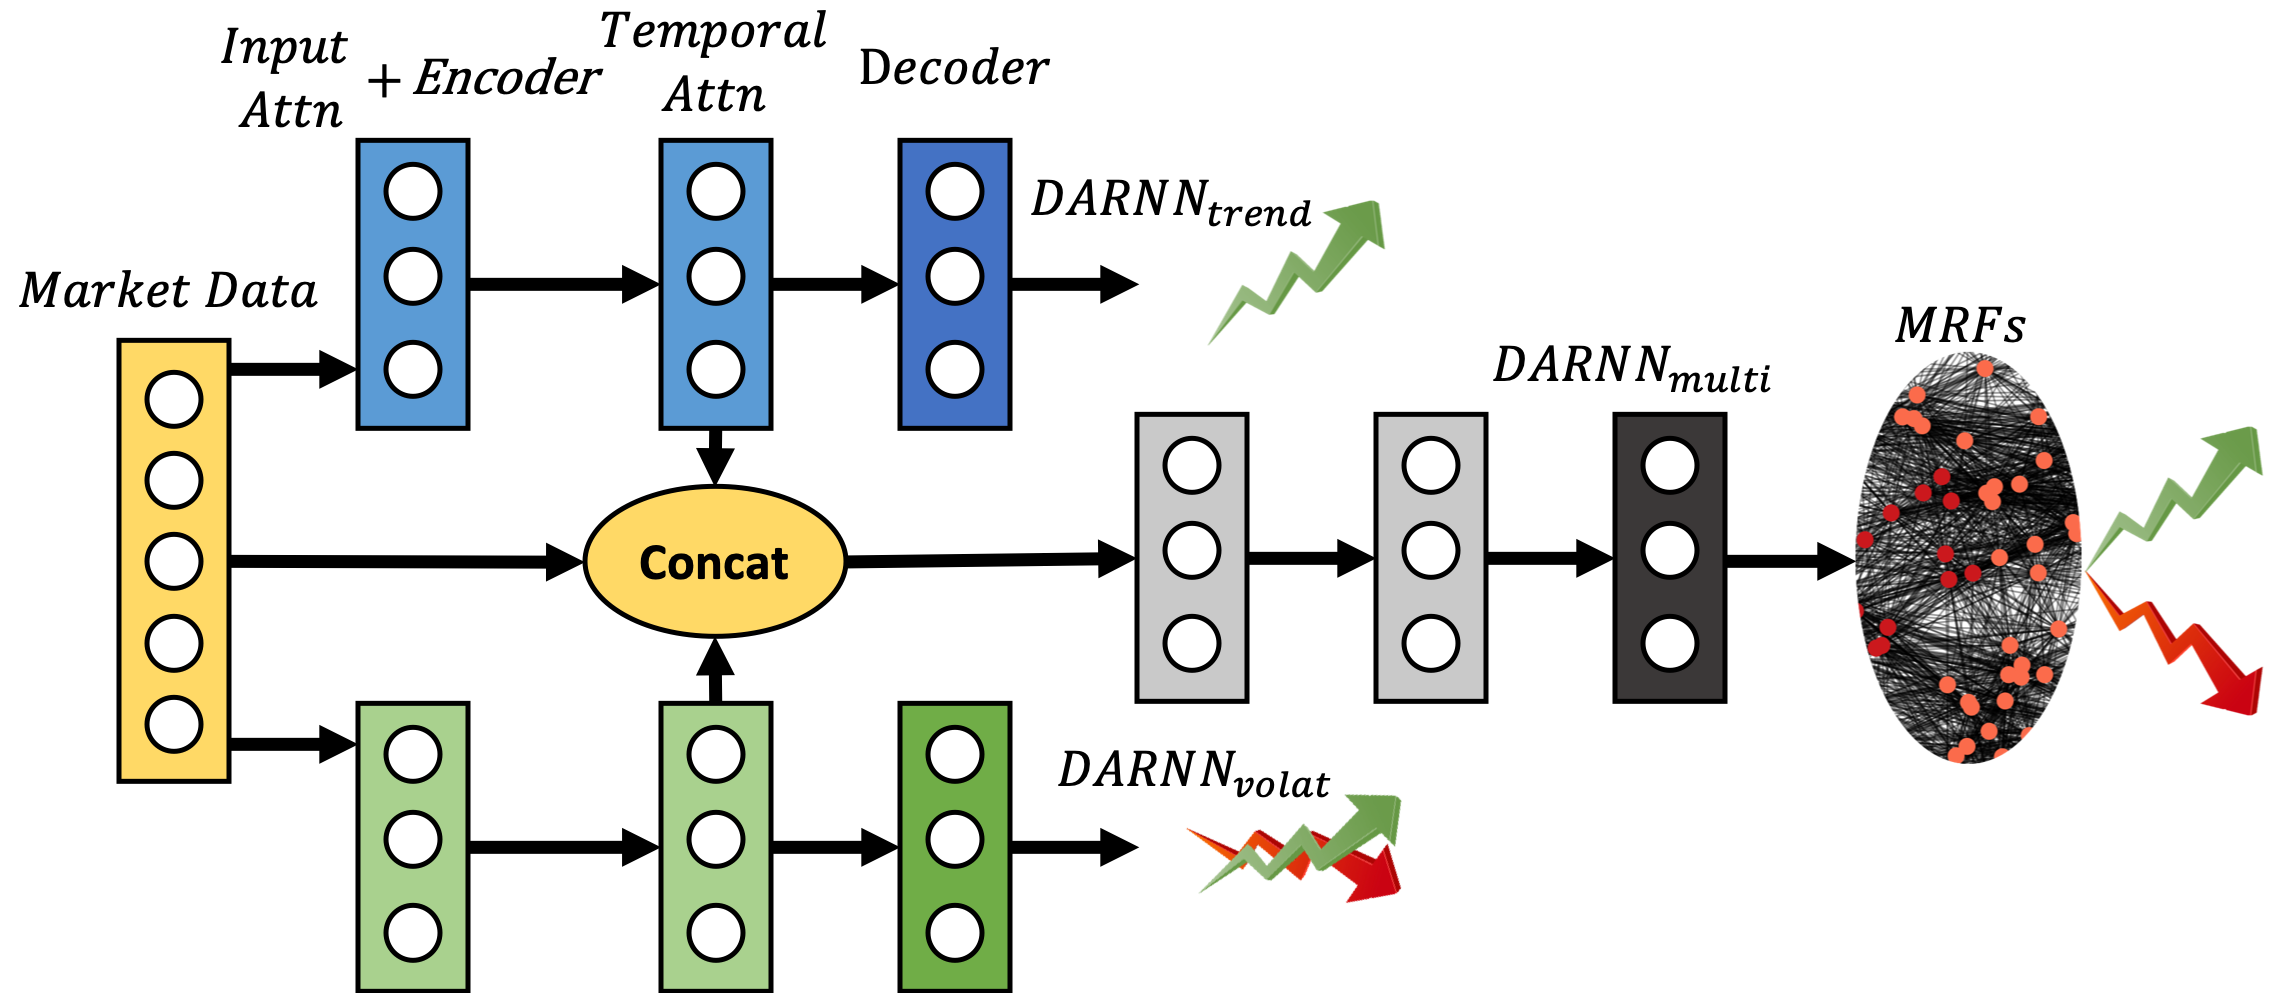
\includegraphics[width=1\columnwidth]{Methodology/figures/hmplmrf.png}
  \caption{\label{fig:mrfrnn} Multi-tasks DNN MRFs Architecture. Note 
  that the output of $\text{DARNN}_{\text{multi}}$ only corresponds to one 
  node's unary feature in MRFs.}
\end{figure}

All three DARNN modules share the same raw market price data.
Here we denote the time-series dataset as $\bX$ where
$\bX=(\bx_1,\bx_2,\dots,\bx_T)\in \reals^{N\times T}$. Here
$\bx^n=(x_1^n,x_2^n,\dots,x_T^n) \in \reals^T$ denotes a driving
series of $T$ time-steps and $\bx_t=(x_t^1,x_t^2\\ ,\dots
,x_t^N)\in \reals^N$ denotes a snapshot at time-step $t$ of all
$N$ features.

For both DARNN modules at the bottom level, the input matrix is a
concatenation of exogenous matrix $\bX \in \reals^{5\times T}$
which contains $5$ exogenous driving series: opening price, low
price, high price, volume, amount and $1$ target series $\by =
(y_1,y_2,\dots,y_T) \in \reals^T$. The task of those DARNNs are
to predict target series $y_{t+p}$ in the next $p$ time steps:

$$\hat{y}_{t+p} = \text{DARNN}(y_1,\dots,y_{t},x_1,\dots,x_t)$$

The target series $\by_{\text{trend}}$ of
$\text{DARNN}_{\text{trend}}$ is closing price. The target series
$\by_{\text{volat}}$ of $\text{DARNN}_{\text{volat}}$ is the
standard deviation of closing price over $M$ time-steps. We use
Mean Squared Error (MSE) as loss function to train those two
modules separately.

To train the top level module, which is a classification DARNN,
we concatenate context vectors $\bc_t$ from each of bottom level
module's second stage encoder and raw market price matrix as
input matrix. The target series $\by^{\text{binary}}$ is
constructed by the sign function $y_t^{\text{binary}} =
sign(y_{t+p}-y_t)$ where $y_t$ denotes closing price at time-step
$t$. We use cross-entropy as loss function to train the final
$\text{DARNN}_{\text{multi}}$. Logits (outputs before going through
\emph{softmax}) of $\text{DARNN}_{\text{multi}}$ are then passed to 
``Sector Rotation Predictor'' as unary features.

In order to train HMPL together with MRFs in an end-to-end manner,
we follow the subgradient method proposed by \citename{witoonchart2017application}.
Since our inner loop proposed in section~\ref{sec:mrflssvm_learning_algo}
is actually a Structural SVM. Only gradients of parameters and feature
functions need to be re-calculated. 
In our framework, outputs of HMPL are only used as unary features in MRFs'
energy functions, our back-propagation rules can be defined by
taking derivative of equation~(\ref{eq:energyfunction_UPH}):

\begin{align}
  \label{eq:der_w}
  \frac{\partial L}{\partial \bw^U} = \psi^U(y)-\psi^U(y^*)
\end{align}

\noindent where $y$ is the ground-truth label and $y^*$ is
inferenced label. And gradients of parameters can be calculated by

\begin{align}
  \label{eq:der_phi}
  \frac{\partial L}{\partial \psi^U} = \bw^U
\end{align}

Equations \eqref{eq:der_w} and \eqref{eq:der_phi} can be directly plugged
into sub-gradient algorithm proposed in \cite{witoonchart2017application}.
Other configurations stay the same with their algorithm.

\subsection{Sector Rotation Predictor}
\label{sec:srp}

We begin with a brief review of our choices of unary, pairwise
and higher-order potential functions. We then show how to perform
exact inference in models with these potentials. In
section~\ref{sec:opt} we will discuss learning the
parameters under the latent structural SVM framework and also how
to back-prop gradients to neural networks.


\subsubsection{Higer Order Energy: The Lower Linear Envelope Function}
\label{sec:llep}

Energy functions can be decomposed over nodes $\N$, edges $\E$
and higher order cliques $\cal C$~\cite{Szummer:ECCV08}. Let
$\bw$ be vector of parameters and $\psi$ be arbitrary feature
function, then the energy can be decomposed as a set of linear
combinations of weights and feature vectors:

\begin{align}
  \label{eq:energyfunction_UPH}
  E(\by;\bw)&=\sum_{i\in \N}{\bw_i^U\psi^U(\by_i)}+ \notag\\
  & \sum_{(i,j)\in \E}{\bw_{ij}^P\psi^P(\by_i,\by_j)}+
  \sum_{\by_C\in \cal C}{\bw_C^H\psi^H(\by_C)}
\end{align}

\noindent where $U$ denotes \emph{unary} terms, $P$ denotes
\emph{pairwise} terms and $H$ denotes \emph{higher order} terms.
In this section we mainly focus on one class of higher-order
potentials $\psi^H$ defined as a concave piecewise linear
function which is known as \emph{lower linear envelope
  potentials}. This has been studied extensively in Markov Random
Fields area for encouraging consistency over large
cliques~\cite{Kohli:CVPR07,Nowozin:2011,Gould:ICML2011}.

Let $\cal C$ denotes the set of all maximal cliques in an image
and $\by_c=\{y_i |\text{\,for\,} i \in C_j\}$ denotes set of
binary random variables where $y_i\in \{0,1\}$ in clique $C_j$, a
weighted lower linear envelope potential over $\by_c$ is defined
as the minimum over a set of $K$ linear functions as:
%
\begin{align}
  \psi^H_c\!(\by_c) \, &= \min_{k=1, \ldots, K} \left\{ a_k W_{\!c}(\by_c) + b_k \right\}.
  \label{eqn:potential2}
\end{align}
%
where $W_{\!c}(\by_c) = \sum_{i \in c} w_i y_i$ with $w^c_i \geq
0$ and $\sum_{i \in c} w^c_i = 1$ which are weights for each
clique. $(a_k, b_k) \in \reals^2$ are the linear function
parameters. We illustrate an example with
four linear functions in \figref{fig:concave}.

\begin{figure}[t]
  \centering
  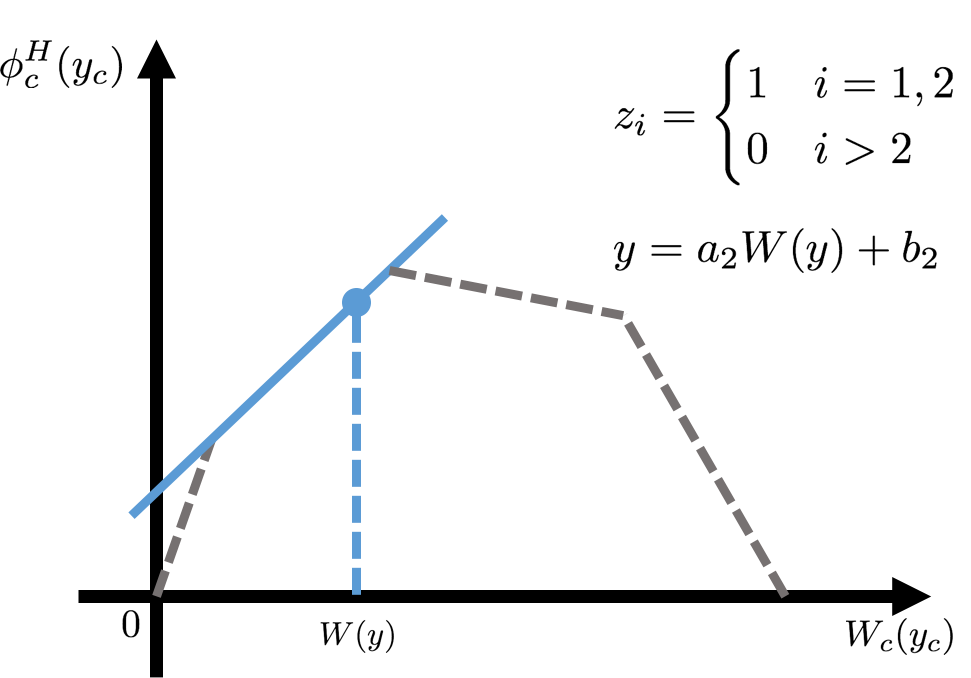
\includegraphics[width=0.8\columnwidth]{Methodology/figures/linEnvLatentFig.png}
  \caption{\label{fig:concave} Example piecewise-linear concave
    function of $W_{\!c}(\by_c) = \sum_{i \in c} w^c_i y_i$.
    Assume the second linear function is active namely
    $\bz^c=(1,1,0,0)$ (equation \ref{eqn:binary_concave_z}). The result of linear combination of
    parameter vector and feature vector is same as quadratic
    psuedo-Boolean function.}
\end{figure}

% % to_replace
% \begin{figure}[ht]
%   \centering
%   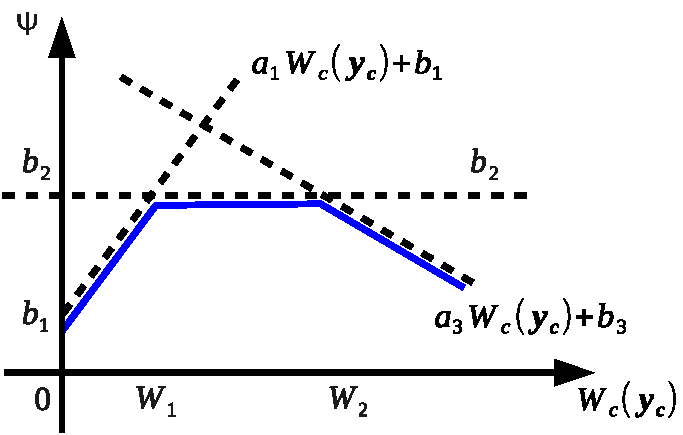
\includegraphics[width=0.6\columnwidth]{Methodology/figures/not_redundant}
%   \caption{\label{fig:nonredundant} Example lower linear envelope
%     $\psi^H_c\!(\by_c)$ (shown solid) with three terms (dashed).
%     When $W_{\!c}(\by_c) \leq W_1$ the first linear function is
%     active, when $W_1 < W_{\!c}(\by_c) \leq W_2$ the second
%     linear function is active, otherwise the third linear
%     function is active.}
% \end{figure}

Inference on energy function contains lower linear potentials is
the same as the standard equation~\eqref{eq:energyfunction_UPH}
and is given by:
\begin{align}
  \label{eq:min_energy}
  \by^* = \argmin\energy{\by}
\end{align}

To ensure potentials do not contain redundant linear functions
(functions that would never be active), \citename{gouldlearning}
proposed a constraint on parameters of the envelope. The $k$-th
linear function is not redundant if the following condition is
satisfied:
%
\begin{align}
    0
    <
    \frac{b_k - b_{k-1}}{a_{k-1} - a_k}
    <
    \frac{b_{k+1} - b_k}{a_k - a_{k+1}}
    <
    1.
  \label{eq:nonredundant}
\end{align}
%
Another important property of equation~\eqref{eq:min_energy} is
shift invariant (vertically). We write
$\widetilde{\psi}^{H}_c\!(\by_c)$ by shift
equation~\eqref{eqn:potential2} vertically with an abitrary
amount $b^{const}\in R$
$$\widetilde{\psi}^{H}_c\!(\by_c) = \min_{k=1, \ldots, K}
\left\{a_k W_{\!c}(\by_c) + b_k + b^\textrm{const} \right\}$$
%
Then we have
\begin{align}
  \argmin_{\by_c} \psi^H_c\!(\by_c)
  = \argmin_{\by_c} \widetilde{\psi}^{H}_c\!(\by_c).
  \label{eq:shift_invariant}
\end{align}
%
Therefore, in the following discussion without loss of generality
we assume $b_1 = 0$ thus $b_k\geq0 \text{\; for \;} k=1,\dots,n$.
%
\subsubsection{Exact Inference}
\label{sec:exact_inference}

Exact inference on MRFs has been extensively studied in past
years. Researchers found that, energy functions which can be
transformed into quadratic pseudo-Boolean
functions~\cite{Ishikawa:PAMI03,Ishikawa:CVPR09,Rother:CVPR09}
are able to be minimized exactly using \emph{graph-cuts} like
algorithms~\cite{Freedman:CVPR05,Hammer:1965} when they satisfy
submodularity condition~\cite{Boros:MATH02}.
\citename{Kohli:TR08} and \citename{Gould:ICML2011} adapted those
results to perform exact inference on lower linear envelope
potentials. In this section we mainly focus on describing the
\emph{st min cut} graph constructed by
Gould~\cite{Gould:ICML2011,gouldlearning} for exact
inference~\eqref{eq:min_energy} of energy function containing
lower linear envelope potentials.

Following the approach of \citename{Kohli:CVPR10},
\citename{Gould:ICML2011,gouldlearning} transformed the weighted
lower linear envelope potential~\eqref{eqn:potential2} into a
quadratic pseudo-Boolean function by introducing $K-1$ auxiliary
variables $\bz = \left(z_1, \ldots, z_{K-1}\right)$ with $z_k\in
\{0,1\}$:

\begin{align}
  E^c(\by_c, \bz) &= a_1 W_{\!c}(\by_c) + b_1 \notag \\
  &+ \sum_{k = 1}^{K-1} z_k \left( \left(a_{k+1} - a_k\right) W_{\!c}(\by_c) + b_{k+1} - b_k \right)
  \label{eqn:binary_concave_z}
\end{align}

\noindent for a single clique $c \in \cal C$. Under this formulation,
minimizing the pseudo-Boolean function over $\bz$ is equivalent
to selecting (one of) the active functions(s) from
equation~\eqref{eqn:potential2}. Another important property of
optimized $\bz$ under this formulation is that it automatically
satisfies the constraint: $z_{k+1} \leq z_k$. This property give rise to further development of
parameter vector and feature
vector (equation~\eqref{eq:llsvm_param} and ~\eqref{eq:llsvm_feature})
which are used in latent
structural SVM.

\begin{figure}[t]
  \centering
  \setlength{\tabcolsep}{2pt}
  \begin{tabular}{cc}
    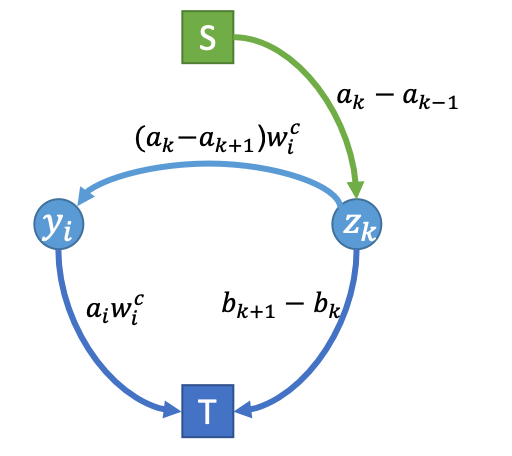
\includegraphics[width=0.54\columnwidth]{Methodology/figures/ho.png}&
                                                                         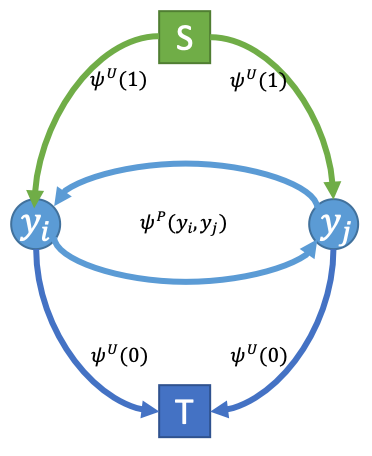
\includegraphics[width=0.4\columnwidth]{Methodology/figures/up.png}\\
                                                                         {\small (a)} & {\small (b)} 
  \end{tabular}
  \caption{\label{fig:stmincut} $st$-graph construction for
    equation~\eqref{eqn:posiform}, unary and pairwise terms.
    Every cut corresponds to an assignment to the random
    variables, where variables associated with nodes in the
    ${\cal S}$ set take the value one, and those associated with
    nodes in the $\T$ set take the value zero. With slight abuse
    of notation, we use the variables to denote nodes in our
    graph.}
\end{figure}



In order to construct the \emph{st-min-cut} graph, we rewrote
equation~\eqref{eqn:binary_concave_z} into
\emph{posiform}~\cite{Boros:MATH02}:

\begin{align}
  \label{eqn:posiform}  
  E^c(\by_c, \bz)
  &= b_1 - (a_1 - a_K) + \sum_{i \in c} a_1 w^c_i y_i \notag\\
  & + \sum_{k = 1}^{K - 1} \left( b_{k+1} - b_k \right) z_k
    + \sum_{k = 1}^{K - 1} \left( a_k - a_{k+1} \right)
    \bar{z}_k\notag\\
  & + \sum_{k = 1}^{K - 1} \sum_{i \in c} \left( a_k - a_{k+1}
    \right) w^c_i \bar{y}_i z_k
\end{align}

\noindent where $\bar{z}_k = 1 - z_k$ and $\bar{y}_i = 1 - y_i$.
$a_1$ is assumed to be greater than $0$ so that all coefficients
are positive (recall we assume $b_1=0$ in section~\ref{sec:llep}
and we have $a_k > a_{k+1}$ and $b_k < b_{k+1}$). Since the energy function~\eqref{eqn:posiform}
is submodular, the \emph{st-min-cut} graph can be constructed 
based on equation~\eqref{eqn:posiform}. The construction (including 
unary and pairwise) is explained in \figref{fig:stmincut}. 

% Figure
% (a) denotes construction for equation~\eqref{eqn:posiform}. For
% each lower linear envelope potential edges are added as follows:
% for each $i \in c$, add an edge from $y_i$ to $t$ with weight
% $a_1 w^c_i$; for each $i \in c$ and $k = 1, \ldots, K-1$, add an
% edge from $z_k$ to $y_i$ with weight $(a_{k} - a_{k+1}) w^c_i$;
% and for $k = 1, \ldots, K-1$, add an edge from $s$ to $z_k$ with
% weight $a_k - a_{k+1}$ and edge from $z_k$ to $t$ with weight
% $b_{k+1} - b_k$. Figure (b) denotes construction for unary and
% pairwise terms (see \cite{Kolmogorov:PAMI04}). For unary edges (4
% edges on both sides), weights on each edge are corresponding to
% values in input unary terms accordingly. For pairwise edges (2
% edges in the middle), both edges share the same weight which
% equals to the input pairwise term.


\section{Optimization}
\label{sec:opt}

\subsection{Transforming Between Representations}
\label{sec:learning}
With the inference algorithm in hand, we now can develop the
learning algorithm for weighted lower linear envelope potentials
using the latent structural SVM framework. We begin by
transforming the equation~\eqref{eqn:binary_concave_z} into a
linear combination of parameter vector and feature vector. Then a
two-step algorithm was developed to solve the latent structural
SVM.

The latent structural SVM formulation requires that the energy
function be formulated into a linear combination of features and
weights while our higher-order potential is represented as the
minimum over a set of linear functions. However,
in~\ref{sec:exact_inference} we reformulated the piesewise linear
functions into a quadratic pseudo-Boolean
function~\eqref{eqn:binary_concave_z} by introducing auxiliary
variables. Now we show function~\eqref{eqn:binary_concave_z}
itself is an inner product of parameter vector and feature vector
with latent information. Note that the function can be expanded
as a summation of $2K-1$ terms:

\begin{align}
  \label{eq:originalenergy}
  E^c(y_c,z)=&a_1W_c(y_c)+b_1\notag \\
            &+\sum_{k=1}^{K-1}z_k((a_{k+1}-a_k)W_c(y_c)+b_{k+1}-b_k)\notag \\ 
            =&a_1W_c(y_c)+\sum_{k=1}^{K-1}(a_{k+1}-a_k)z_kW_c(y_c) \notag \\
            &+\sum_{k=1}^{K-1}(b_{k+1}-b_k)z_k
\end{align}

Here we use the fact of equation~\eqref{eq:shift_invariant} and
let $b_1=0$. Now we can reparameterize the energy function
as
\begin{align}
  \label{eq:llsvm_innerprod_energy}
  E^c(\by_c,\bz; \btheta) = \btheta^T \! \psi(\by_c,\bz)
\end{align}

\noindent where:

\begin{equation}
\label{eq:llsvm_param}
  \theta_k = \left\{
    \begin{aligned}
      & a_1	& \text{for} \ k=1\\
      & a_k-a_{k-1} & \text{for}\ 1< k \leq K\\
      & b_{k+1-K}-b_{k-K} & \text{for} \ K<k\le2K-1\\
    \end{aligned}
  \right.
\end{equation}

\begin{equation}
\label{eq:llsvm_feature}
  \psi_k = \left\{
		\begin{aligned}
      & W_c(\by_c) 	& \text{for} \ k=1\\
      & W_c(\by_c)\bz_k & \text{for}\ 1<k\le K\\
      & \bz_k & \text{for} \ K<k\le2K-1\\
		\end{aligned}
  \right.
\end{equation}

Under this formulation, inference problems in
\cite{yu2009learning} can be written as:

\begin{align}
  \label{eq:linenv_full_inf}
  (\mathbf{\hat{y}}_k(\btheta),\mathbf{\hat{z}}_k(\theta))=\argmin_{(\mathbf{y}
  \times \mathbf{z}) \in \mathcal{Y} \times \mathcal{Z}}
  \btheta^T\cdot\psi(\mathbf{y}_k,\mathbf{z}_k)
\end{align}
and
\begin{align}
  \label{eq:linenv_latent_inf}
  \mathbf{z}^*_k(\btheta) = \argmin_{\mathbf{z} \in \mathcal{Z}}
  \btheta^T \cdot \psi(\mathbf{y}_k,\mathbf{z}_k)
\end{align}

There are 2 facts worth to mention. The first fact is
that in our previous construction of minimum-$st$-cut graph the
latent variable $\bz$ is already included. Therefore, we can
apply our inference algorithm directly on our 2 new formulations.

More interesting for equation~\eqref{eq:linenv_latent_inf} there exists
more efficient algorithm. At training stage the ground-truth
labels $y_i$ is a function input thus completely observed.
Therefore, the term $((a_{k+1}-a_k)W_c(\by_c)+b_{k+1}-b_k)$ in
equation~\eqref{eq:originalenergy} becomes constant. So we can
infer latent variable $\bz$ explicitly by:
\begin{align}
  \label{eq:linenv_effi_infer_latent}
  z_k^c &=
          \begin{cases}
            0 & \text{if $((a_{k+1}-a_k)W_c(y_c)+b_{k+1}-b_k)\geq0$} \\
            1 & \text{otherwise}.
          \end{cases}
\end{align}

Therefore, assignments inferred by graph-cut algorithm can be
directly encoded into a linear combination by using our latent
structural SVM formulation for learning purpose. The remaining
task is to ensure the concavity of $\btheta$. We do this by
adding following constraint:

\begin{align}
  \label{eq:concave_constraint}
  A\btheta\geq\epsilon \text{,\;~~~} A=
                  \begin{bmatrix}
                    1 & \mathbf{0} & \mathbf{0}\\
                    \mathbf{0} & -\mathbf{1} & \mathbf{0}\\
                    \mathbf{0} & \mathbf{0} & \mathbf{P}
                  \end{bmatrix}\in \mathbb{R}^{(2K-1)\times(2K-1)}
\end{align}

\noindent where $-\mathbf{1}$ is a matrix of size $(K-1)\times(K-1)$ and
$\mathbf{P}$ is an identity matrix of size $(K-1)\times(K-1)$.
One subtle problem we found during experiments is that the
algorithm can be stuck with small numerical value. To avoid this
we add small slack variables $\epsilon=\mathbf{1}^{-15}$ on 
those constraints.

\subsection{Latent Structural SVM Learning}
\label{sec:mrflssvm_learning_algo}

\begin{algorithm}
  \begin{algorithmic}[1]
    \STATE{Set $MaxIter = 100$}
    \STATE{ {\bf input} training set $\{\by_i\}_{i=1}^{n}$, regularization constant $C > 0$,
      and tolerance $\epsilon \geq 0$}
    \STATE{Initialize $\btheta$ using \algref{alg:init_theta}}
    \REPEAT \STATE{CCCP Outer Loop}
    \STATE{Set $iter = 0$}
    \FOR{each training example, $i = 1, \ldots, n$}
    \STATE{compute $ \bz_i^*=\argmax_{\mathbf{z} \in \mathcal{Z}}
      \theta \cdot \psi(\mathbf{y}_i,\mathbf{z}) $}
    \ENDFOR

    \STATE{ {\bf initialize} active constraints set ${\cal C}_i = \{ \}$ for all $i$}
    \REPEAT \STATE{CCCP Inner Loop}

    \STATE{solve the quadratic programming problem in
      equation~\ref{eq:mrflssvm_object} with respect to active
      constraints set ${\cal C}_i$ for all $i$ and concavity constraints
      $A\btheta\geq \epsilon$ to get
      $\hat{\btheta}$ and $\hat{\bxi}$}

    \FOR{each training example, $i = 1, \ldots, n$}
    \STATE{compute $\hat{\by_i},\hat{\bz_i} = \argmin_{\by}
      E(\by,\bz; \hat{\btheta}) - \Delta(\by, \bz, \by_i)$}
    \IF{$\hat{\xi}_i + \epsilon \!<\! \Delta(\hat{\by_i},
      \hat{\bz_i}, \by_i) -
      E(\hat{\by_i},\hat{\bz_i}; \hat{\btheta}) + E(\by_i, \bz_i^*; \hat{\btheta})$}
    \STATE{${\cal C}_i \leftarrow {\cal C}_i \cup \{{\by}_i^\star\}$}
    \ENDIF
    \ENDFOR
    \UNTIL{no more violated constraints}
    \STATE{ {\bf return} parameters $\hat{\btheta}$}
    \STATE{Set $iter = iter+1$}

    \UNTIL{$iter\geq MaxIter$}
    \STATE{ {\bf return} parameters $\hat{\btheta}$}
  \end{algorithmic}
  \caption{\label{alg:learning} Learning lower linear envelope
    MRFs with latent variables.}
\end{algorithm}

With the inner product formulation
(equation~\eqref{eq:llsvm_innerprod_energy}) of higher order
energy function in hand, we now able to develop our latent
structural SVM learning algorithm. The energy function (higher
order function together with unary and pairwise functions) can be
written as:
\begin{equation}
  E_{all}(y,z) = \begin{bmatrix}
    \btheta^H\\
    \theta^{unary}\\
    \theta^{pairwise}
  \end{bmatrix}^T 
  \cdot \begin{bmatrix}
    \psi^H\\
    \psi^{unary}\\
    \psi^{pairwise}
  \end{bmatrix}=\theta_{all}^T\cdot\psi_{all}
\end{equation}
where $\btheta^H\in \reals$ is the parameter vector in higher
order equation~\eqref{eq:llsvm_innerprod_energy} of size $2K-1$.
$\theta^{unary}$ and $\theta^{pairwise}$ are both scalars.
$\psi^\textrm{unary} = \sum_i \psi^U_i\!(y_i)$ and
$\psi^\textrm{pairwise} = \sum_{ij} \psi^P_{ij}(y_i, y_j)$.
Therefore, the size of $\theta_{all}$ is $2K+1$.

% Plug equation~\eqref{eq:linenv_full_inf} and
% equation~\eqref{eq:linenv_latent_inf} into object function in
% \cite{yu2009learning}, the latent structural SVM object function
% for our problem can be derived as a difference of two convex
% functions:

% \begin{align}
% \label{eq:lssvm_object}
%   \min_\theta\bigg(\frac{1}{2}\|\theta\|^2+
%   C\sum_{i=1}^{n}\big(\max_{(\mathbf{\hat{y}} \times
%   \mathbf{\hat{z}}) \in \mathcal{Y} \times \mathcal{Z}}
%   [\theta\cdot\psi(\mathbf{\hat{y}},\mathbf{\hat{z}}) +
%   \Delta(\mathbf{y}_i,\mathbf{\hat{y}},\mathbf{\hat{z}})]\big)\bigg)\\
%   -C\sum_{i=1}^{n}\big(\max_{\mathbf{z} \in \mathcal{Z}} \theta \cdot
%   \psi(\mathbf{y}_i,\mathbf{z})\big)\nonumber
% \end{align}

Following \citename{yu2009learning}, we use the two stages Concave-Convex
Procedure (CCCP)~\cite{yuille2002concave} to solve the
optimization problem. We first
imputes the latent variables $\bz$ explicitly by
equation~\eqref{eq:linenv_latent_inf}. Namely solving the
``latent variable completion'' problem~\cite{yu2009learning}:

\begin{align}
  \bz_i^*=\argmax_{\mathbf{z} \in \mathcal{Z}} \theta \cdot
  \psi(\mathbf{y}_i,\mathbf{z})
\end{align}

The inference result $z_i^*$ for $i=1,\dots,n$ is used as
completely observed for later stage. With the latent variable
$z_i^*$ which best explains the ground-truth data $y_i$ in hand,
updating the parameter vector $\btheta$ reduces to solve the
standard structural SVM problem:

\begin{align}
\label{eq:mrflssvm_object}
  \min_\theta\bigg(\frac{1}{2}\|\theta\|^2+
  C\sum_{i=1}^{n}\big(\max_{(\mathbf{\hat{y}} \times
  \mathbf{\hat{z}}) \in \mathcal{Y} \times \mathcal{Z}}
  [\theta\cdot\psi(\mathbf{\hat{y}},\mathbf{\hat{z}}) +
  \Delta(\mathbf{y}_i,\mathbf{\hat{y}},\mathbf{\hat{z}})]\big)\bigg)\\
  -C\sum_{i=1}^{n}\big(\theta \cdot
  \psi(\mathbf{y}_i,\mathbf{z}_i^*)\big) \nonumber
\end{align}

Our optimization algorithm is summarized in
\algref{alg:learning}. As we mentioned in \appref{sec:train_detail}, 
although we proposed an end-to-end
subgradient algorithm is section \ref{sec:hmpl}, MRFs updated by
such algorithm take too many iterations to converge. Therefore,
we propose a two-stage training procedure. At first stage, HMPL
and MRFs are trained separately. Therefore, MRFs can take
advantage of the efficient latent structural SVM and converge in
a polynomial number of iterations. After all those models are
converged, we then combine them together to conduct end-to-end
training. Note that the CCCP Inner Loop in \algref{alg:learning}
is actually solving standard structural SVM problem. Therefore,
at the second stage, we use subgradient algorithm proposed in
section~\ref{sec:hmpl} to replace the CCCP Inner Loop. Other
settings remain the same.

The last problem remaining is the initialization method. Because
our objective function~\eqref{eq:mrflssvm_object} is not convex
and the CCCP algorithm is only guaranteed to converge to a local
minimum or saddle point\cite{yuille2002concave}, initialization
of $\btheta$ might affect the performance of our algorithm. Since
there are no theoretical solution for this problem, we propose an
empirical initialization algorithm in \appref{sec:sup_init}.


\section{Experiment}
\label{sec:exp}

In this section, we first introduce 3 stock datasets (index) and
how we use them to construct our final input datasets. Then, we
introduce the parameter settings of our model and other training
details. Finally, we select four evaluation metrics and use them
to demonstrate our framework's effectiveness by comparing with
several baseline methods.

\subsection{Dataset and Model Settings}
\label{sec:dataset}

To demonstrate the effectiveness of higher order consistency, we
choose three exclusive and the most famous stock indexes on Chinese
stock market to build our input datasets. Their index codes are:
CSI (China Securities Index) 200, CSI 300 and CSI 500 which
contain 200, 500 and 300 constituent stocks respectively. The CSI
300 index selects most liquid A-share stocks. It aims to reflect
the overall performance of China A-share market. The CSI 200 and
500 index aims to reflect the overall performance of mid-to-large
and small-to-mid capital A-shares respectively.

All these indexes are exclusive and are refined on a yearly
basis. In this paper, we use fixed versions on 30-JAN-2015. We
then collect their constituent stocks' minute-level data from
05-JAN-2015 to 29-DEC-2017. On Chinese stock market each trading
day has 3 trading hours. So there are 240 samples for each
normally traded stock each day. Each sample contains 6 features:
opening price, high price, low price, closing price, volume,
amount. \footnote{During this period, there are some stocks
  de-listed (SZ000024, SH600485, SH600832 in CSI 200; SZ000693,
  SZ000748, SZ000982 in CSI 500; SH600485, SH600832, SZ000024,
  SH601299 in CSI 300). Therefore, in total we collect 197, 497
  and 296 stocks during this period respectively.} For each
stock, the first $80\%$ days are used to construct the training
set and the last $20\%$ days are used as testing set.
Approximately training set and testing set contain 13 million and
3 million samples, respectively.

\begin{table}[H]
\centering
\small
\caption{Technical Indicators Selection}
\begin{tabular}{|c|c|} \hline
  Category&Indicator Name\\ \hline
  Momentum& Awesome Oscillator, Money Flow Index\\ \hline
  Volume& \makecell{Chaikin Money Flow\\ On-balance volume mean}\\ \hline
  Volatility& Bollinger Bands (Upper and Lower Bands)\\ \hline
  Trend& \makecell{Average Directional Movement Index\\Moving Average Convergence Divergence}\\ \hline
\end{tabular}
  \label{tab:ta}
\end{table}

To demonstrate benefits of multi-task RNN over
manually designed technical indicators, we also need to construct
technical indicators datasets for each of those market price
dataset collected above. We select 8 most popular indicators, 2
from each category~\cite{kirkpatrick2010technical} shown in Table
\ref{tab:ta}. In implementation, we use open source package
\emph{Technical Analysis Library in
  Python\footnote{https://github.com/bukosabino/ta}} to calculate
those indicators and all hyper parameters are using package's
default settings. After technical indicators calculation, these 8
new features are concatenated to above market price dataset (5
features at each minute). So the final input dataset for each single
task model contains 13 features in total. Before feeding into
models, we normalize each stock with \emph{z-score}
function using standard deviation and mean calculated in the training set.

For brevity, we denote market price dataset which only contains  $5$ features as \textbf{Market} and the concatenated $13$ features dataset as
\textbf{Indicator}. As discussed in section~\ref{sec:hmpl}, 
closing price at time $t$ can be directly used as regression 
target for $\text{DARNN}_{\text{trend}}$. 
Standard deviation of closing price with a window size of $10$ 
is used as regression target for $\text{DARNN}_{\text{volat}}$.
The dimensions of
hidden state and cell state are 32 for $\text{DARNN}_{\text{trend}}$ as well as $\text{DARNN}_{\text{volat}}$ and
128 for $\text{DARNN}_{\text{multi}}$. More training details are
described in appendix \ref{sec:train_detail}.

\subsection{Results}
\label{sec:res}

In order to demonstrate the effectiveness of our framework, we
run 3 baselines on 3 different Chinese Securities Indexes with
and without technical analysis indicators as inputs. Results are
summarized in Table~\ref{tab:result}. All results are reported over the test sets. We select four metrics as evaluation
metrics to justify the effectiveness of the proposed approach. They are calculated by collecting all
predicted labels of constituent stocks in each CSI index.

\begin{table*}[t]
\centering
\small
\setlength\tabcolsep{2pt}
\caption{Results: Baselines and ablation study. All models have a
  window size (lag steps) of 20 and predict price movement label
  at the next time step.}
\begin{tabular}{@{}cccccccccccccc@{}}
\toprule
Data Set                   & Models                          & \multicolumn{12}{c}{Chinese Securities Index (CSI)}                                                                                                                                                                                                    \\ \midrule
\multicolumn{2}{c}{\multirow{2}{*}{}}                        & \multicolumn{4}{c}{CSI200}                                                                & \multicolumn{4}{c}{CSI500}                                                             & \multicolumn{4}{c}{CSI300}                                        \\
\multicolumn{2}{c}{}                                         & Accuracy                   & Precision      & Recall         & F1 Score                   & Accuracy       & Precision      & Recall         & F1 Score                            & Accuracy       & Precision      & Recall         & F1 Score       \\ \cmidrule(r){1-2} \cmidrule(lr){4-5} \cmidrule(lr){8-9} \cmidrule(lr){12-13}
\multirow{3}{*}{\textbf{Indicator}} & LSTM                            & 62.30                      & 73.82          & 70.70          & 72.23                      & 60.35          & 68.56          & 70.03          & 69.29                               & 60.16          & 71.39          & 68.50          & 69.91          \\
                           & \multicolumn{1}{c|}{LSTM\_ATTN} & 64.26                      & 72.41          & \textbf{74.34} & \multicolumn{1}{c|}{73.36} & 61.13          & 75.63          & 66.67          & \multicolumn{1}{c|}{70.86}          & 64.26          & 75.54          & 70.57          & 72.97          \\
                           & DARNN                           & 63.09 & 72.08          & 73.55          & 72.81                      & 66.60          & 78.98          & \textbf{74.13}          & \textbf{76.48}                               & 65.82          & 76.68          & 73.46          & 75.04          \\ \cmidrule(r){1-2} \cmidrule(lr){4-5} \cmidrule(lr){8-9} \cmidrule(lr){12-13}
\multirow{5}{*}{\textbf{Market}}    & LSTM                            & 57.62                      & 67.57          & 67.37          & 67.47                      & 55.86          & 68.10          & 64.53          & 66.27                               & 56.25          & 67.17          & 65.98          & 66.57          \\
                           & \multicolumn{1}{c|}{LSTM\_ATTN} & 59.57                      & 71.60          & 66.86          & \multicolumn{1}{c|}{69.15} & 58.40          & 69.53          & 68.12          & \multicolumn{1}{c|}{68.81}          & 61.33          & 71.87          & 68.91          & 70.36          \\
                           & \multicolumn{1}{c|}{DARNN}      & 61.13                      & 71.26          & 71.47          & \multicolumn{1}{c|}{71.37} & 63.09          & 77.04          & 67.87          & \multicolumn{1}{c|}{72.16}          & 63.87          & 72.09          & 73.59          & 72.83          \\
                           & \multicolumn{1}{c|}{HMPL}       & 65.04                      & 74.04          & 73.39          & \multicolumn{1}{c|}{73.72} & 65.43          & 76.04          & 72.80 & \multicolumn{1}{c|}{74.38} & 66.60          & 71.67          & \textbf{78.90} & 75.11          \\
                           & HMPL+MRFs                       & \textbf{67.97}             & \textbf{77.51} & 73.91          & \textbf{75.67}             & \textbf{66.80} & \textbf{79.65} & 72.78          & 76.06                               & \textbf{68.95} & \textbf{78.55} & 74.71          & \textbf{76.58} \\ \bottomrule
\end{tabular}
\label{tab:result}
\end{table*}

\subsubsection{Effectiveness of multi-task framework}

As mentioned earlier, to demonstrate effectiveness of multi-task
framework, we use \textbf{Indicator} dataset, which contains both
market price data and technical analysis indicators as inputs for
DARNN and \textbf{Market} dataset which only contains market
price data as inputs for HMPL and other single task models. For
vanilla DARNN, we use a hidden size of $128$. HMPL's
configuration is described in section~\ref{sec:multi_train}. As
we can see in Table~\ref{tab:result}, single task models (LSTM,
LSTM\_ATTN, DARNN) tested on \textbf{Market} dataset (without
technical analysis indicators as inputs) generally have worse
performance on all 4 metrics. In particular, performance of DARNN
models tested on \textbf{Indicator} dataset is consistently
better than the ones on \textbf{Market} dataset. This proves that
even with hand-crafted features, deep learning models can still
benefit from diversified and complementary features. By comparing
DARNN tested on \textbf{Indicator} and HMPL on \textbf{Market},
we can see that HMPL marginally outperforms DARNN on CSI200 and
CSI300 index constituent stocks and is slightly worse on CSI500
constituent stocks. We can conclude that by using multi-task
RNN, we can extract equally good features compared with
hand-crafted features.

\subsubsection{Effectiveness of higher-order MRFs}

In Table 2, we can observe that HMPL-MRFs framework consistently outperforms other baselines on all 3 CSI index constituent stocks. It shows evidence that higher-order energy function can help with
encoding clique level consistency thus improving overall
prediction performance. One interesting point to note is that the recall rate of HMPL-MRFs is constantly lower than other baselines. This can be seen as a trade off between accuracy and recall rate. However, it is worth to mention that for stock price movement prediction, high accuracy and precision are much preferred than recall rate. Another interesting phenomenon is that HMPL-MRFs gives higher improvements on CSI200 and CSI300 while little improvements over DARNN trained with technical
analysis indicators on CSI500. One possible reason is that CSI200 and CSI300 select most liquid and representative stocks in Chinese stock market. Those stocks exhibit much stronger and higher order consistency than illiquid stocks. CSI500 selects small-mid
capital stocks which are less liquid and contains much more noisy movements.

\subsubsection{Visualization of higher-order consistency}

In order to further investigate higher-order MRFs' effectiveness,
we design a heat-map to visualize CSI300 index intra-clique
higher-order relationship in figure~\ref{fig:consistency}.

\begin{figure*}[t]
  \centering
  \setlength{\tabcolsep}{20pt}
  \begin{tabular}{ccc}
  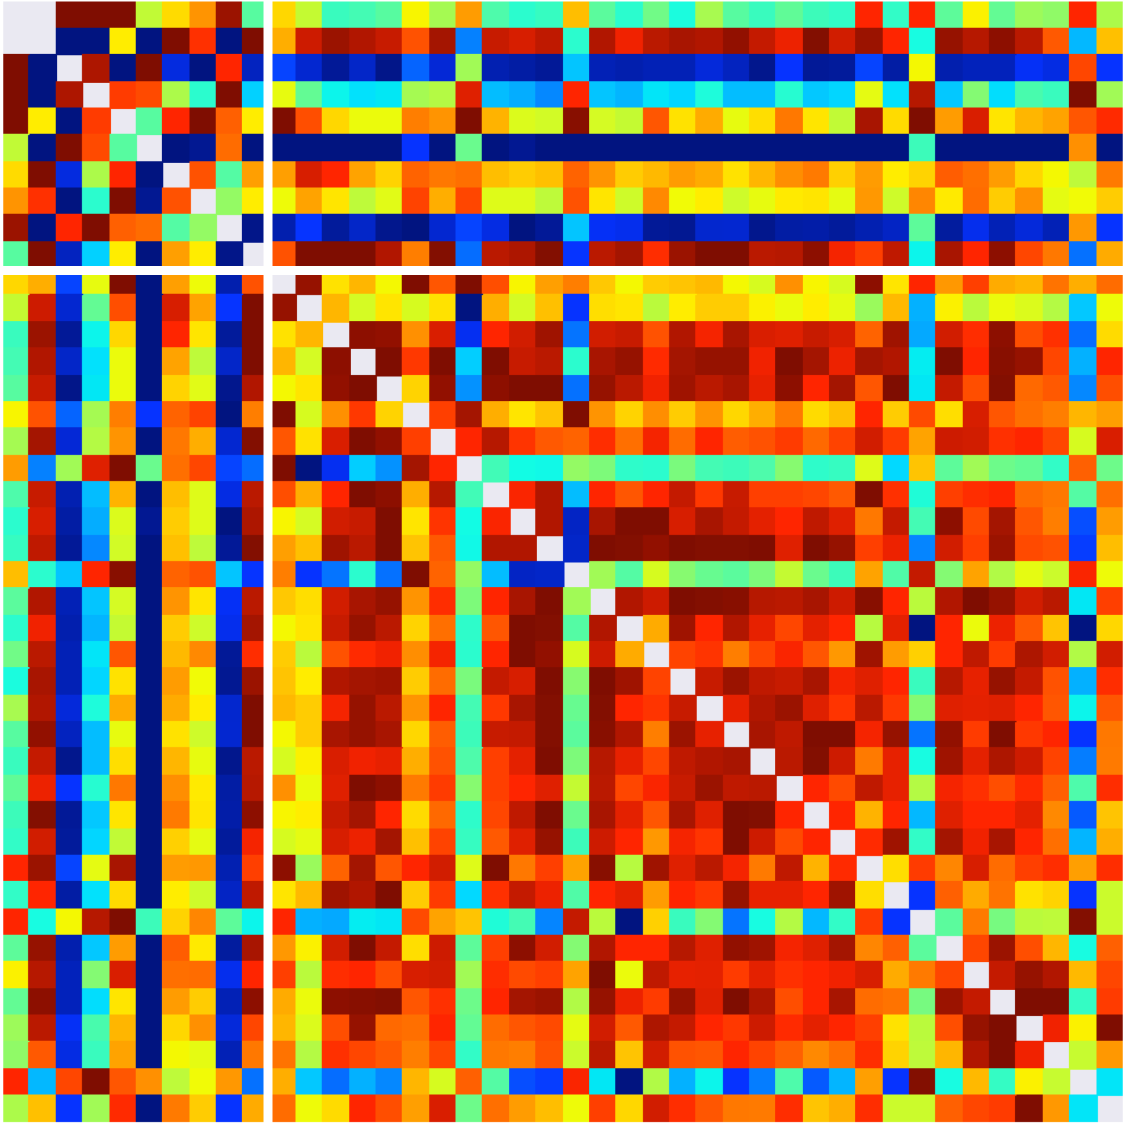
\includegraphics[width=0.45\columnwidth]{Methodology/figures/gt.png}&
  

    
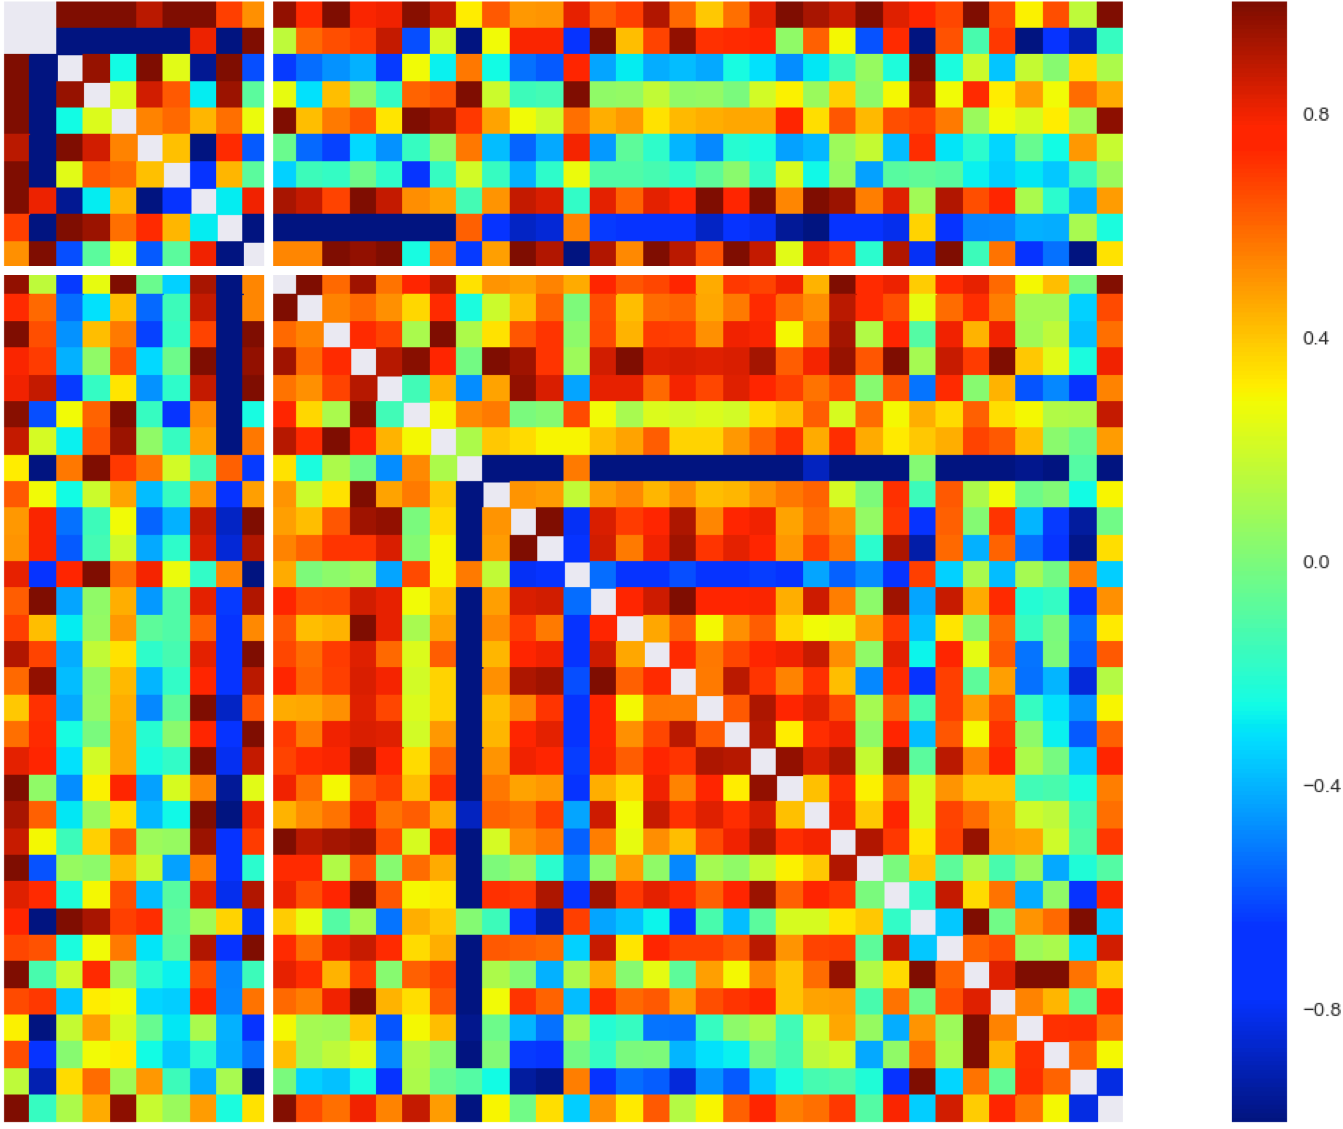
\includegraphics[width=0.54\columnwidth]{Methodology/figures/hmpl.png}&

    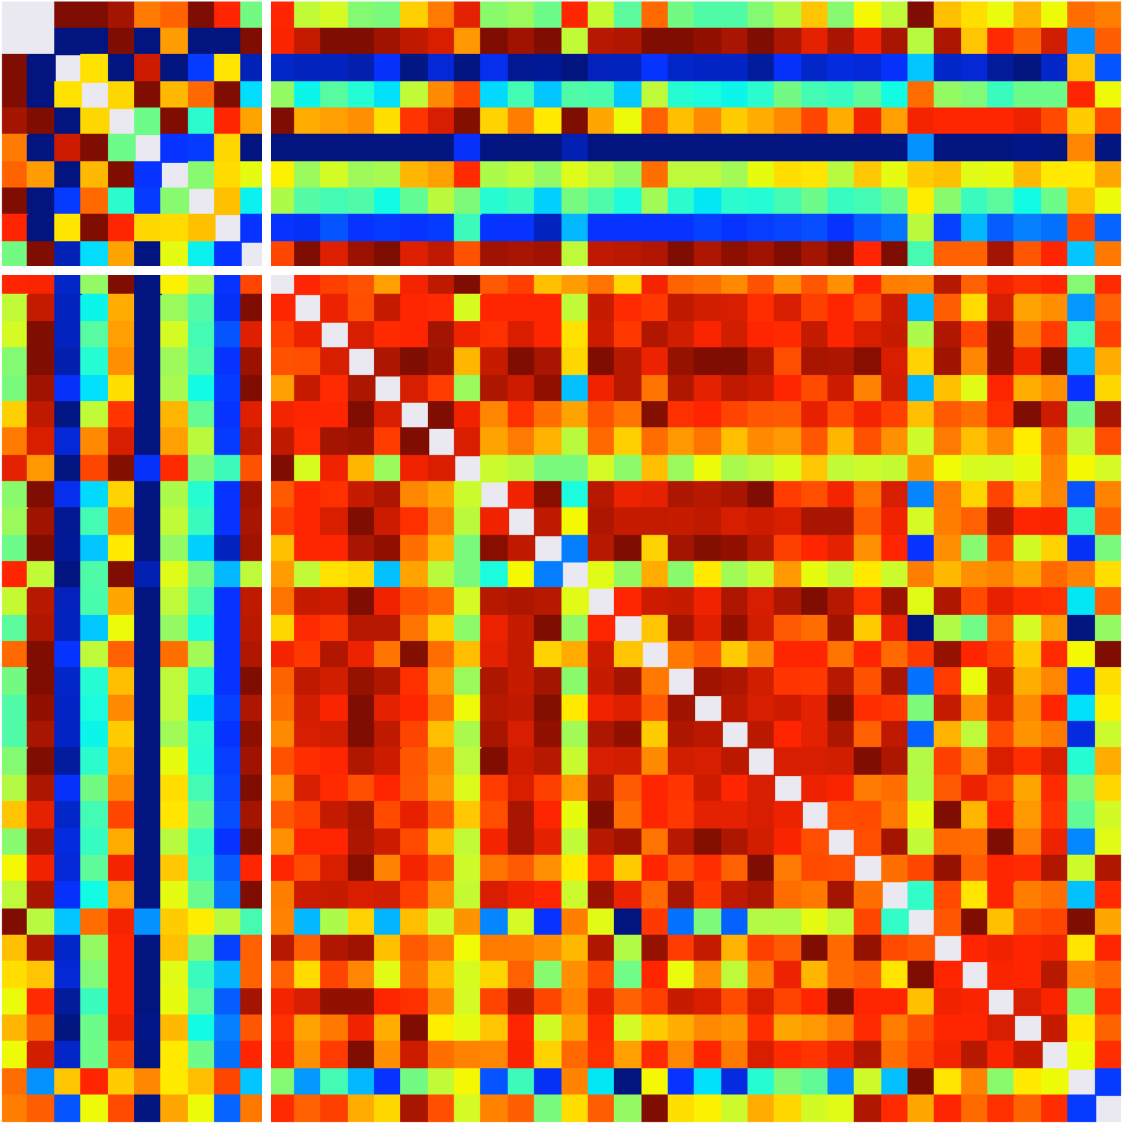
\includegraphics[width=0.45\columnwidth]{Methodology/figures/mrf.png}
\\                                                                        {\small (a) Ground-truth} & {\small (b) HMPL } & {\small (c) HMPL-MRFs} 
  \end{tabular}\vspace{-2mm}
  \caption{\label{fig:consistency} Higher order consistency
    visualization. Figure (a) is calculated
    directly from ground truth labels on test set.
    Figure (b)
    is calculated using predicted labels of HMPL without MRFs on the
    test set.
    In figure (c), we use predicted labels of
    HMPL-MRFs on test set as inputs.}\vspace{0mm}
\end{figure*}

We first select two sectors: nonferrous metal sector, which
contains 10 constituent stocks, and infrastructure sector, which
contains 35 constituent stocks from CSI300 index \footnote{These
  two sectors are selected only because painting many sectors in
  one figure would be too messy to interpret and those two
  sectors have appropriate clique size (number of stocks) for
  visualization. Conclusions from these two sectors also apply to
  other sectors}. We then measure consistency level between each
two of these constituent stocks. In order to capture their
temporal relationship, we propose a novel consistency measure
which is calculated on temporal intervals.
% Let $\C\in\{\text{Nonferrous Metal},\text{Infrastructure}\}$
% denotes one clique. $\by_c=\{\by_i \in \C\}$ denotes a set of
% time-series $\by_i^T=\{y_i^1,y_i^2,...,y_i^T\}$ for all stocks

Let $\by_i^T=\{y_i^1,y_i^2,...,y_i^T\}$ denotes time-series for
stock $i$. $y_i^t\in \{0,1\}$ is the binary price movement label
at time $t$. We segment time-series $\by_i^T$ into
$N=\lceil\frac{T}{P}\rceil$ non-overlapping intervals
$\{y_i^n,y_i^{n+1},...,y_i^{n+P}\}$ with fixed length $P$. For
any two stocks $i$ and $j$, we calculate the difference
$d_{ij}^n=\sum_n^{n+P}{y_i^n}-\sum_n^{n+P}{y_j^n}$ of how many
times positive price movement happen in the $n$th time interval
in each stock. Then the consistency level $c_{ij}$ between stocks
$i$ and $j$ can be calculated as a $\ell_1\text{norm}$:
$$c_{ij}=-\|\mathbf{d}_{ij}\|_1$$
\noindent where
$\mathbf{d}_{ij}=\{d_{ij}^1,d_{ij}^2,...,d_{ij}^N\}$. We
normalize $c_{ij}$ into interval $[-1,1]$. Each entry in
figure~\ref{fig:consistency} denotes a consistency level measure
$c_{ij}$. The larger the $c_{ij}$ is, the higher of consistency
level between stock $i$ and stock $j$, the color of corresponding
entry is closer to red, and vice versa. As we mentioned, the average duration of information
arrival-conduction-integration-release process is 4.04 minutes.
Since which stock is leading at each time interval is elusive, we
set $P=9$ when calculating consistency measures.

As we can see in figure (a), there is a significant red square
area, which means ground-truth heat-map shows strong intra-clique
consistency. This is an evidence that higher-order relationships
do exist within clique of stocks. However, in figure (b), the red
square area is fragmented into many little pieces. The whole
area's color is closer to blue when compared to ground-truth
heat-map, which means that HMPL captures little higher-order consistency.
The reason we still can observe a shape of red square
is that the accuracy of HMPL model on CSI300 is $66.6\%$.
However, we can still conclude that the accuracy of single HMPL
model mainly comes from unary features and it fails to capture
higher order consistency relationships lies in clique of stocks.
On the contrary, even though HMPL-MRFs model's accuracy on CSI300
index is only $2.35\%$ better than HMPL model, we can observe
that heat-map (c) is more close to ground-truth heat-map than
heat-map (b). There is a much clear red square and the number of
small fragments in red area is also less than figure (b). We can
conclude that HMPL-MRFs models learn to utilize both unary
features from HMPL as well as higher-order relationships encoded
in MRFs.

\vspace{-3mm}
\section{Conclusion}
\label{sec:conc}

This paper has shown how to model individual stock price
prediction problem without hand-crafted features and encode
lead-lag relationships among stocks using weighted higher-order
MRFs. A multi-task neural networks framework, Holistic Market
Price Learner (HMPL) is proposed to automatically extract
diversified and complementary features from individual stock
price sequence. Features learned by HMPL are passed to a binary
MRFs with weighted lower linear envelope energy function to
utilizing intra-clique higher order consistency among stocks. An
efficient latent structural SVM algorithm is designed for
learning MRFs in polynomial time. Finally the MRFs and HMPL are
trained end-to-end using sub-gradient algorithm. Extensive
experiments are conducted on three major index on Chinese stock
market. The proposed HMPL-MRFs achieves best accuracy on all
three indexes.

Our work gives insights to a number of directions for future
research. One obvious extension is to apply our method to a multi-label
MRFs to help with 3-classes price movement prediction. A More interesting direction is to investigate the implicit relationship between the expert defined index list and Graph RNN \cite{you2018graphrnn}. Investigating under this direction could help further diminishing domain knowledge required by our framework.



\bibliographystyle{ACM-Reference-Format}
%\bibliographystyle{plainnat}
\bibliography{Bibs/thesis,Bibs/long,Bibs/scene,Bibs/proposal,Bibs/fin}

\newpage

\appendix

\section{Training Details}
\label{sec:train_detail}

\subsection{Initialization of lower linear envelope}
\label{sec:sup_init}

We assume that the more evenly distributed of $W_c(Y_c)$ where
$c\in\cal C$ on $x$ axis, the more rich representation (number of
linear functions) the energy function should have. In order to
initialize $\btheta$, we first determine the x-coordinate of
sampled points $sp$. Then we sample its y-coordinate from a
uniform distribution ${\cal U}(\text{upbound},\text{upbound}-0.5)$ to add some
randomness in our initialization as well as maintain concavity.
Linear parameters $a_k$ and $b_k$ are later calculated using
those sampled points $sp_k$ and $sp_{k-1}$. At last we encode
$\{a_k,b_k\}_{k=1}^K$ into $\btheta$ using
equation~\eqref{eq:llsvm_param}. This algorithm is summarized in
\algref{alg:init_theta}.

\begin{algorithm}[h]
  \begin{algorithmic}[1]
    \STATE{$gap=\frac{1}{K}$, $a_1={\cal U}(0,1e6)$, $b_1=0$,
      $sp_1=(0,0)$, $w_0=0$, $counter=2$} \FOR{each
      clique $c\in \cal C$} \STATE{Compute weighted clique value
      $w_c=W_c(y_C)$} \IF{$w_c-w_{c-1}>gap$}
    \STATE{$upbound = a_{counter}w_c+b_{counter}$\\
      $sp_{counter}=(w_c,{\cal U}(upbound-0.5,upbound))$\\
      Calculate $a_{counter}$ and $b_{counter}$ using
      $sp_{counter-1}$ and $sp_{counter}$\\
      $counter=counter+1$}
    \ENDIF
    \ENDFOR
    \STATE{If $counter<K$, remaining $a$s and $b$s are all set to
      be $a_{counter}$ and $b_{counter}$} \STATE{Calculate
      $\btheta$ using $\{a_k,b_k\}_{k=1}^K$}
  \end{algorithmic}
  \caption{\label{alg:init_theta} Empirical initialization
    algorithm for $\btheta$}
\end{algorithm}

\subsection{Multi-task training}
\label{sec:multi_train}

To improve accuracy and reduce over-fitting, we add a drop out
layer between input layer and LSTM layer with a ratio of $0.2$.
We also clip and normalize gradients during back-propagation
stage with a maximum norm of $5.0$ to prevent gradient exploding
issue. As pointed out by \citename{lample2016neural}, the
question of ``when should the training schedule switch from one
task to another task?'' or ``should each task be weighted
equally?'' remains open. In our implementation, we follow the
proportional sampling approach described by
\citename{sogaard2016deep}. After a backward pass completed, we
randomly sample a new task as well as its batch data as the next
task to be trained. In practice, we use a proportion of
$[0.25,0.25,0.5]$ for three tasks respectively. This mechanism
helps multi-task model to avoid \emph{Catastrophic Forgetting}
phenomenon which means lower level model forgets learned
knowledge during higher level model back-propagation pass.

Even though we propose an end-to-end training algorithm for HMPL
and MRFs in section~\ref{sec:hmpl}, MRFs inference stage is still
too slow to be trained jointly with HMPL. To overcome this
difficulty, we implement a two stages training procedure. We
first add a \emph{softmax} layer on top of
$\text{DARNN}_{\text{class}}$ and train HMPL separately from
MRFs. We use \emph{Negative Log-likelihood} as the loss function.
At the second stage, after HMPL converge, we remove the
\emph{softmax} layer and re-train it together with MRFs. One
issue we must mention is that, even though we use binary MRFs
which can only predict positive / negative price movement, we
find there is a significant amount of time when stock price
remains no change. We find it benefits the performance a lot if
we treat the classification as a three classes problem rather
than a binary classification problem during the first stage.
Therefore, at the first stage, the \emph{softmax} layer will
output probability for three labels: \emph{negative movement},
\emph{no changes} and \emph{positive movement}. Since binary MRFs
still needs a two dimension input as part of unary energy
function, after the \emph{softmax} layer is removed, we add an
additional linear mapping layer between logits of HMPL and MRFs
at the second stage.

\subsection{End-to-end NN-MRFs training}
\label{sec:mrf_train}

With converged HMPL and MRFs at hand, now we can go forward to train
them in an end-to-end manner. We only include pairwise energy function through
section~\ref{sec:srp} and section~\ref{sec:opt} to show a general
application of our proposed algorithm. In the case of Chinese
stock market, to our best knowledge there is no public available
definition of pairwise relationship between stocks. Therefore, in
our implementation we only use unary and higher order energy
function. Each stock is then treated as a node in MRFs and each
stocks group which has lead-lag relationships is treated as a
maximum clique in MRFs. One benefit of MRFs clique is that we can
embed domain expert knowledge about industry classification as
maximum cliques into our model. We choose to use Tonghuashun
industry classification \cite{ths} in our model. One subtle but
crucial detail about modeling lead-lag effect lies in
equation~(\ref{eqn:potential2}). Recall that $W_{\!c}(\by_c) =
\sum_{i \in c} w_i y_i$ with $w^c_i \geq 0$ and $\sum_{i \in c}
w^c_i = 1$ which are weights for stocks in each clique.
Therefore, leading stocks should have a higher weights while
lagging stocks should have lower weights. In our implementation,
we use constituents' weight defined in CSI200, CSI500 and CSI300
as their weights in equation~(\ref{eqn:potential2}) and normalize
them to ensure the summation equals $1$.



% That's all folks!
\end{document}
